\section{Training scenario}
\label{ch1:sec:training}
\begin{figure}
    \centering
    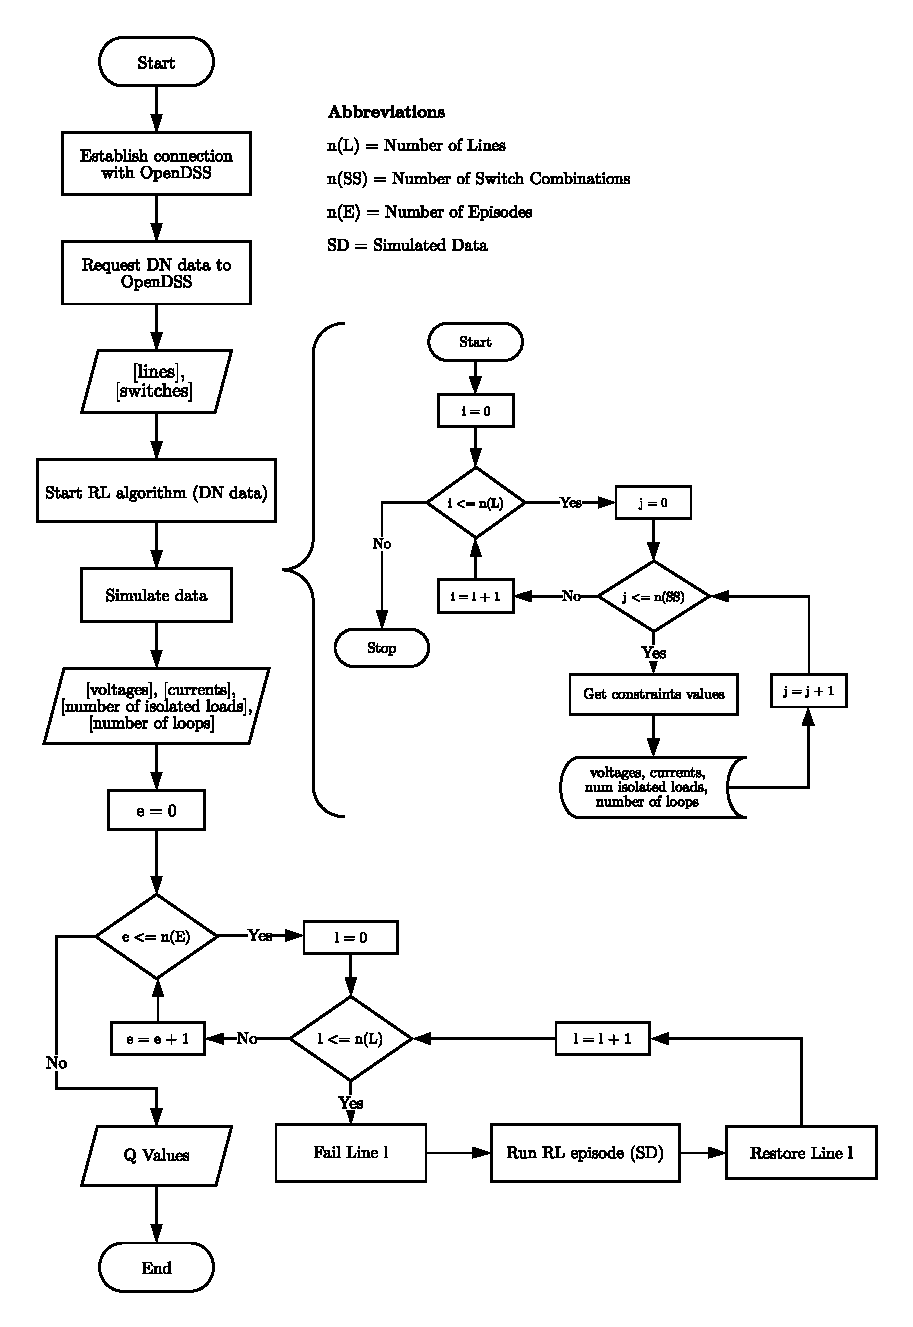
\includegraphics[scale=0.9]{_chapter1/fig/training_scenario.pdf}
    \caption{SR Algorithm - Training Scenario}
    \label{ch1:fig:training_blocks}
\end{figure}

The restoration algorithm starts with Training scenario, which is presented in Figure \ref{ch1:fig:training_blocks}. 
In there, the SR algorithm establishes a connection with OpenDSS and requests the lines and switches data. 
Then, it initializes the RL class with lines and switches passed as a parameter. 

Henceforth, the RL class handles the SR algorithm processes. First, it co-simulates with OpenDSS to obtain the voltage and current profiles, the number of isolated loads, and the number of loops for all possible switch status and faulted line combinations. This simulated data is stored in .ftr files and loaded into the SR algorithm.

Secondly, an episode begins: a line is selected and faulted. So, the RL object performs interactions between the agent and the environment until the environment reaches the terminal state, which is the optimal state after a fault event. 
Once the terminal state is reached, the RL algorithm restores the faulted line and repeats the aforementioned process by selecting a new line to fail. 

This must be done for all lines and during a fixed number of episodes. 

As a result, the Q value matrix stores the optimal SR plan, and the training is completed. 
